\documentclass[addpoints,12pt]{exam}
%\documentclass[12pt]{article}
\usepackage[letterpaper, margin=0.75in]{geometry}
\usepackage{graphicx}
\usepackage{enumitem}
\usepackage{booktabs}
\usepackage{tabularx}
\usepackage{color}

\begin{document}
\footer{}{Page \thepage\ of \numpages}{}

\begin{flushright}
\makebox[0.5\textwidth]{\large Name:\enspace\hrulefill}
\vspace{0.2in}

\makebox[0.5\textwidth]{\large Date:\enspace\hrulefill}
\end{flushright}

\begin{center}

\includegraphics[width=10cm]{../images/logo.png}
\end{center}

\begin{center}
\noindent{\LARGE Conceptual Physics \\ Homework Packet 4\\}
\end{center}


\noindent \noindent\begin{large}\textbf{Due: April 20, 2018}\end{large}
\vspace{0.2in}

The content in this homework relates to material covered in class 9 (atomic/particle theory and light) and 10 (fields of force).
\begin{enumerate}
	\item \textit{Light and Matter}, Chapter 17 (Sections 1)
	\item \textit{Light and Matter}, Chapter 19 (Sections 3 and 4)
	\item \textit{Light and Matter}, chapter 26 (Sections 1 and 4)
	\item \textit{Light and Matter}, Chapter 22 (Sections 1 to 3):
\end{enumerate}

\begin{center}
	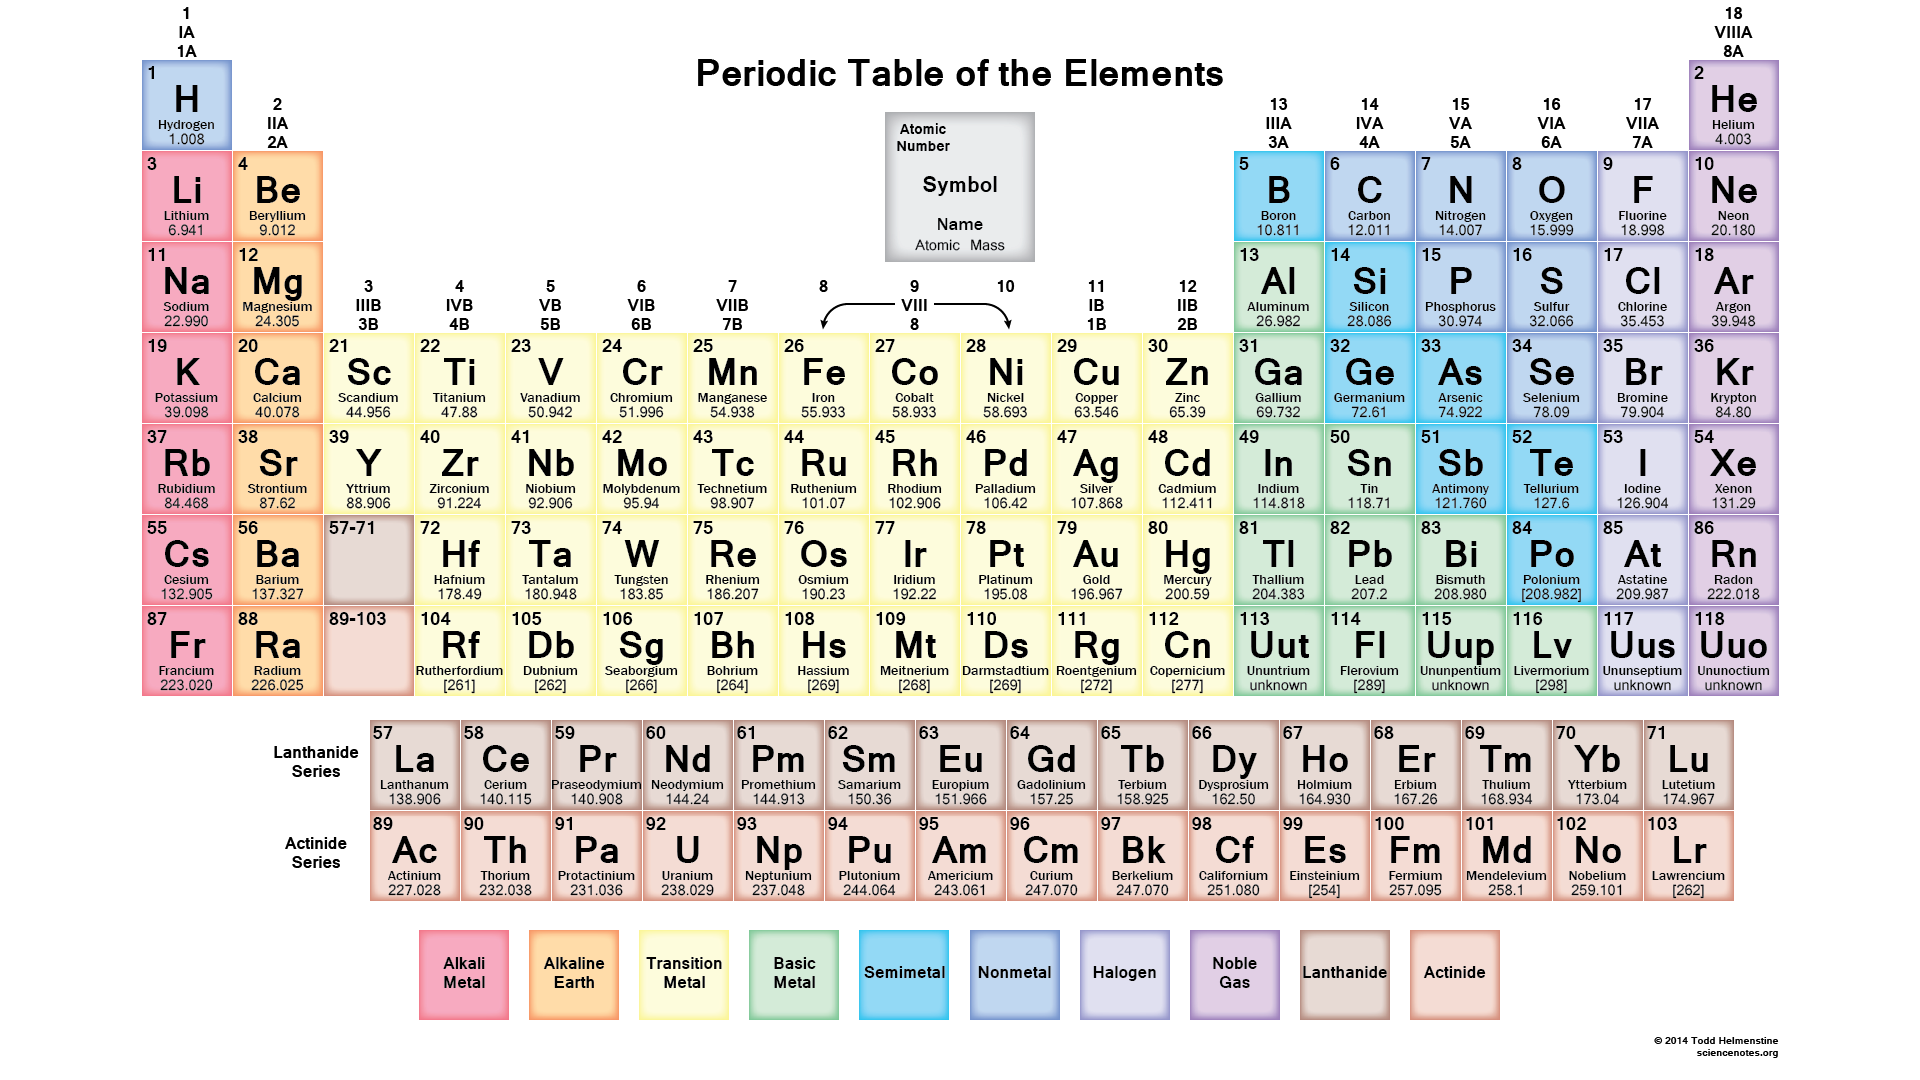
\includegraphics[width=\textwidth]{../images/periodicTable.png}
\end{center}
 
\clearpage

\begin{flushright}
Score: \hspace{0.2in} / \numpoints ~ points
\end{flushright}

\begin{questions}
	
\question[6]
\begin{parts}
	\part What is the difference between an \textit{elementary} and a \textit{composite} particle?
		\vspace{0.5in}
	\part List 2 \textit{elementary particles}:
		\vspace{0.5in}
	\part List 2 \textit{composite particles}:
		\vspace{0.5in}
\end{parts}

\question[6] Plutonium-240 ($Pu^{240}$) decays by emitting a helium-4 nucleus.
	\begin{parts}
		\part How many protons are in plutonium-240?
			\vspace{0.5in}
		\part How many neutrons are in plutonium-240?
			\vspace{0.5in}
		\part When a plutonium-240 nucleus decays and emits a helium-4 nucleus, what element does it turn into? How many protons and neutrons are in this nucleus?
			\vspace{0.5in}
	\end{parts}
	
	\question[4] Primordial light from the big bang continues to exist in our universe, but it has been highly \textit{red-shifted} due to the universe's expansion, to the point that it is in the microwave region. This is known as the \textit{cosmic microwave background} (CMB) and physicists are highly interested in measuring it because we can use it as a probe of the early universe.
	\begin{parts}
		\part In the past, was the \textit{frequency} of the CMB greater, smaller or the same as it is now?
			\vspace{0.5in}
		\part In the past, was the \textit{wavelength} of the CMB greater, smaller or the same as it is now?
			\vspace{0.5in}
	\end{parts}
	
	\clearpage
	\question[10] There is a gravitational field surrounding the Earth and Moon.
	\begin{parts}
		\part Using field lines, draws the gravitational field around the Earth and Moon.
			\vspace{1in}
			\begin{center}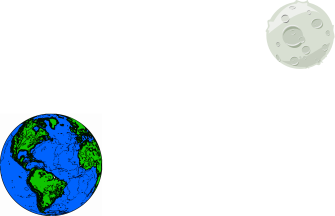
\includegraphics[width=2in]{../images/earthMoon.png}\end{center}
			\vspace{1in}
			
		\part Using a ``field of arrows", draw the gravitational field around the Earth and Moon.
			\vspace{1in}
			\begin{center}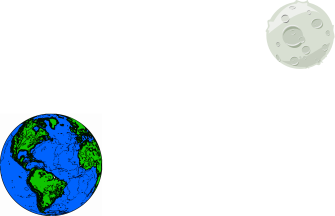
\includegraphics[width=2in]{../images/earthMoon.png}\end{center}
			\vspace{1in}
			
		\part There is a point at which the gravitational field is zero. Indicate this point on each of the above diagrams for part (a) and (b).
		\part What force would a test mass experience at the location where the gravitational field is zero?
	\end{parts}
	
	\clearpage
	\question[6] When you stand on the surface of the Earth, you experience the full strength of its gravitational field.
	\begin{parts}
		\part What happens to the strength of this gravitational field, if you were to dig deep into the Earth? (Does it increase, decrease, or stay the same?) Please explain your reasoning. Hint: Think about what is generating the gravitational field, and think about the pull of the earth beneath and \textit{above} you as you did deeper.
			\vspace{2in}
		\part What is the strength of the Earth's gravitational field, at the center of the Earth?
			\vspace{2in}
		\part From this reasoning, draw the gravitational field (as arrows or lines, whichever you prefer) for a hollow sphere using the cross-section provided bellow.
			\vspace{1in}
			\begin{center}
			
\includegraphics[width=1.5in]{../images/hollow.png}
			\end{center}
	\end{parts}
	
\end{questions}








\end{document}